\newcommand{\ClassPath}{../../VIU_TFM_LaTeX_template}
\documentclass{\ClassPath/viu-tfm-template}
\usepackage{multicol}

\definecolor{maincolor}{HTML}{e65218}

%--------------------------------------------------------------------------
% Definiciones necesarias Modifica con tus datos
%--------------------------------------------------------------------------
\def\nombre{Gómez Olivencia, Rubén}
\def\dni{78910013-A}
\def\titulo{Análisis y diseño de la aplicación web \linebreak\linebreak\linebreak para la Asociación Internacional de Chefs}
\def\titulacion{Máster Universitario en Desarrollo de Aplicaciones y Servicios Web}
\def\curso{2022-2023}

%Los siguientes son opcionales: si no se ponen, la portada cambia un poco. Ideal para escribir artículos/trabajos cortos
\def\dirige{}
\def\convocatoria{}
\def\asignatura{Ingeniería Software Web}


% importar fichero de Bibliografía
\addbibresource{Actividad_2.bib}

\begin{document}
    \graphicspath{{../../VIU_TFM_LaTeX_template/}}

    \coverpage

    \tableofcontents

\chapter{Introducción}
En el siguiente documento se va a detallar el camino utilizado para la realización de la aplicación web solicitada por la  \textbf{Asociación Internacional de Chefs (AIC)} para la gestión y compartición de recetas culinarias.

A lo largo del documento se diferenciarán distintos apartados en los que se detallarán cuál ha sido la metodología empleada durante todo el proceso, la planificación realizada y cómo se ha hecho la obtención y posterior análisis de requisitos.

Con todo ello, se ha realizado el modelado de datos que es necesario para llevar a cabo la petición del cliente, así como distintos diseños conceptuales que serán explicados en sus respectivos apartados.

Para finalizar se han incluido las conclusiones de todo el proceso llevado a cabo.


\chapter{Metodología utilizada}
Para llevar a cabo la creación de la aplicación web, y todo el proceso subyacente, se ha hecho uso del método “diseño centrado en el usuario” (\textbf{DCU}), y tal como nos dice la definición de \textcite{hassan2004diseno} “se caracteriza por asumir que todo el proceso de diseño y desarrollo del sitio web debe estar conducido por el usuario, sus necesidades, características y objetivos”.

Es por eso, que para llevar a buen puerto el proyecto encargado por la \textbf{AIC}, debemos de comprender las funcionalidades presentadas y sus requerimientos buscando como objetivo final el tener la mejor experiencia de usuario.

\chapter{Planificación}
Antes de comenzar con los requisitos del proyecto, y con el objetivo de tener un mejor entendimiento y comunicación con la \textbf{AIC}, se ha realizado una planificación para definir el alcance del proyecto.

De esta manera, podemos decir, tal como se dice en el lenguaje coloquial, que estamos todos los involucrados en el proyecto (tanto el cliente \textbf{AIC}, como los analistas y desarrolladores que hemos llevado a cabo el proyecto) en la misma página.

No está de más recordar que el objetivo común es llevar a buen término el proyecto de creación de la aplicación web de recetas.

\section{Alcance del proyecto}
Aunque se detallarán más adelante de manera más granular los requisitos obtenidos, a continuación se expone la premisa principal del alcance del proyecto (en lo que se refiere a funcionalidad) y cuál es el deseo por parte de \textbf{AIC} en este proyecto:

\vspace{-1em}
\begin{enumerate}[label=\alph*)]
    \item Registrar el usuario a la plataforma de la AIC.
    \item Autenticar usuario al ingresar a la aplicación de la AIC.
    \item Cargar la receta, con todos sus aspectos asociados (categoría, lista de
    ingredientes, procedimiento, dificultad, costo, etc.)
    \item Buscar recetas en base a distintos aspectos: clase de receta, tipo de ingrediente
    de base, nivel de dificultad, costo de la receta.
    \item Visualizar resultados de búsqueda.
    \item Visualizar la información sobre cada receta.
    \item Compartir receta en las redes.
    \item Valorar receta (de 1 a 5 estrellas).
\end{enumerate}
\vspace{-1em}

Todo ello se realizará bajo una aplicación en entorno web, cuyos usuarios objetivos son \textbf{personas adultas de toda Europa y América}.


Como ya se ha comentado, esto son los \textit{items} principales que se pretenden conseguir y que posteriormente serán analizados en detalle.



\chapter{Requisitos del cliente}

En este apartado vamos a detallar cómo se ha realizado toda la toma de requisitos y el análisis para poder realizar una diferenciación de los mismos para su posterior modelado, tanto de datos como de interfaces.

Antes de continuar, cabe recordar qué es un requisito, y tal como nos dice \textcite{Sommerville2005} “es una declaración abstracta de alto nivel de un servicio que debe proporcionar el sistema o una restricción de éste”.

Así mismo, y teniendo en cuenta la definición proporcionada por la \textcite{IEEE610} en su estándar 610.12-1990, se define como “una condición o capacidad que debe estar presente en un sistema o componentes de sistema para satisfacer un contrato, estándar, especificación u otro documento formal”.


\section{Obtención de los requisitos}
Para la obtención de los requisitos se realizaron una serie de entrevistas con los responsables de la \textbf{AIC} con el fin de recabar toda la información posible para que de esta manera quedasen claro las funcionalidades y requisitos mínimos que debe tener la aplicación web.

A la reunión acudieron los responsables de negocio de la Asociación Internacional de Chefs (\textbf{AIC}) y por otro lado, en función de analista, Rubén Gómez Olivencia.



\section{Análisis de requisitos}
Una vez realizadas las reuniones con los responsables de \textbf{AIC} el paso llevado a cabo ha sido el de analizar toda la información recabada para pasar a formalizar los requisitos que debe cumplir el proyecto.

Este análisis ha sido diferenciado en las siguientes categorías:

\vspace{-1em}
\begin{itemize}
    \item Requisitos de negocio
    \item Requisitos funcionales
    \item Requisitos no funcionales
    \item Requisitos del sistema
\end{itemize}

En cada uno de los diferentes apartados de este documento se explicarán el alcance de cada una de las categorías.


\subsection{Requisitos de negocio}
Desde la \textbf{AIC} el requisito de negocio es el darse a conocer, y para ello quieren crear la aplicación a la que invitar a todos lo interesados en el arte culinario a subir sus recetas, valorar las recetas de otros usuarios y compartirlas a través de sus redes sociales.


\subsection{Requisitos funcionales}
Para que entendamos qué son los requisitos funcionales \textcite{Sommerville2005} nos propone la definición de que son las declaraciones de los servicios que debe proporcionar el sistema. En definitiva, cómo se va a comportar el sistema en distintas situaciones que tengamos en él.

Los requisitos funcionales engloban distintos apartados que vamos a ver a continuación y en los que iremos detallando cada uno de los requisitos obtenidos.


\subsubsection{Requisitos transaccionales}
Los requisitos transaccionales los podemos resumir como las funcionalidades que tendrá la aplicación, así como las tareas que el usuario podrá realizar con los datos contenidos en la aplicación.

En base a estos requisitos transaccionales y estas funcionalidades, veremos cómo posteriormente surgirán nuevos requisitos (como pueden ser los requisitos de datos y requisitos de interfaz).

\newcounter{reqno}
\setcounter{reqno}{1}


\begin{requisitostbl}{X[-1]X[1]X[1]X[1]X[1]}
    ID & Tipo & Categoría & Prioridad &  Dependencias \\
    \arabic{reqno}  & Funcional & Transaccional & Must &    \\

    Registro de usuarios  \\

    \textbf{Descripción}:

    La plataforma permitirá el registro del usuario solicitando los siguientes datos:
    \begin{multicols}{2}
        \begin{itemize}
            \item E-mail
            \item Contraseña
            \item Nombre y apellidos (opcional)
            \item Fecha de nacimiento
            \item Género (opcional)
            \item País (opcional)
        \end{itemize}
    \end{multicols}
    \vspace{-2em}
    \\

    \textbf{Razón}:

    Para poder registrar recetas el usuario debe estar registrado en el sistema.  Algunos datos son opcionales. La fecha de nacimiento es obligatoria ya que los usuarios deben ser mayores de edad.\\
\end{requisitostbl}

\stepcounter{reqno}


\begin{requisitostbl}{X[-1]X[1]X[1]X[1]X[1]}
    ID & Tipo & Categoría & Prioridad &  Dependencias \\
    \arabic{reqno}  & Funcional & Transaccional & Must &  1  \\

    Autenticación de usuarios  \\

    \textbf{Descripción}:

    La plataforma solicitará los siguientes datos para autenticar un usuario:
    \begin{multicols}{2}
        \begin{itemize}
            \item E-mail
            \item Contraseña
        \end{itemize}
    \end{multicols}
    \vspace{-2em}
    \\

    \textbf{Razón}:

    Para poder realizar ciertas acciones (crear recetas) el usuario debe estar autenticado\\
\end{requisitostbl}

\stepcounter{reqno}


\begin{requisitostbl}{X[-1]X[1]X[1]X[1]X[1]}
    ID & Tipo & Categoría & Prioridad &  Dependencias \\
    \arabic{reqno}  & Funcional & Transaccional & Must &  2  \\

    Registrar nueva receta  \\

    \textbf{Descripción}:

    El sistema permitirá a los \textbf{usuarios \underline{registrados}} que registren nuevas recetas, solicitando los siguientes datos:
    \begin{multicols}{2}
        \begin{itemize}
            \item Nombre de la receta
            \item Ingredientes
            %            \item Puntuación (otorgada por el resto de usuarios, sólo al visualizarla)
            \item Categoría de receta
            \item Nivel de dificultad (de 1 a 5)
            \item Coste de preparación
            \item Procedimiento de elaboración
            \begin{itemize}
                \vspace{-0.6em}
                \item Texto
                \item Multimedia: fotos [opcional]
                \item Multimedia: vídeo [opcional]
            \end{itemize}
        \end{itemize}
    \end{multicols}
    \vspace{-2em}
    \\

    \textbf{Razón}:

    Las recetas deben contener esos datos para posteriormente buscar por ellos, o para poder visualizarlos. La inserción de fotos o vídeo es opcional y se podrá realizar a través de la misma web.\\
\end{requisitostbl}


\stepcounter{reqno}


\begin{requisitostbl}{X[-1]X[1]X[1]X[1]X[1]}
    ID & Tipo & Categoría & Prioridad &  Dependencias \\
    \arabic{reqno}  & Funcional & Transaccional & Must &    \\

    Búsqueda de recetas  \\

    \textbf{Descripción}:

    El sistema permitirá realizar búsquedas de recetas en base a los siguientes criterios:
    \begin{multicols}{2}
        \begin{itemize}
            \item Clase de receta
            \item Tipo de ingrediente base
            \item Nivel de dificultad
            \item Coste de la receta (precio máximo y mínimo)
        \end{itemize}
    \end{multicols}
    \vspace{-2em}
    \\

    \textbf{Razón}:

    Para que los usuarios puedan buscar recetas, se les permitirá hacerlo usando varios criterios.\\
\end{requisitostbl}


\stepcounter{reqno}

\begin{requisitostbl}{X[-1]X[1]X[1]X[1]X[1]}
    ID & Tipo & Categoría & Prioridad &  Dependencias \\
    \arabic{reqno}  & Funcional & Transaccional & Must & 4   \\

    Visualizar los resultados de búsquedas \\

    \textbf{Descripción}:

    El sistema permitirá visualizar el resultado de las búsqueda realizadas para poder elegir una receta en concreto.
    \\
\end{requisitostbl}

\stepcounter{reqno}

\begin{requisitostbl}{X[-1]X[1]X[1]X[1]X[1]}
    ID & Tipo & Categoría & Prioridad &  Dependencias \\
    \arabic{reqno}  & Funcional & Transaccional & Must & 3   \\

    Visualizar la información de la receta \\

    \textbf{Descripción}:

    El sistema permitirá visualizar todos los datos (de manera ordenada) de una receta seleccionada.

    \\

    \textbf{Razón}:

    Esta es la funcionalidad principal de la aplicación junto con el ingreso de recetas.
    \\
\end{requisitostbl}


\stepcounter{reqno}

\begin{requisitostbl}{X[-1]X[1]X[1]X[1]X[1]}
    ID & Tipo & Categoría & Prioridad &  Dependencias \\
    \arabic{reqno}  & Funcional & Transaccional & Must & 6   \\

    Compartir receta en redes sociales \\

    \textbf{Descripción}:

    El sistema permitirá compartir una receta a través de las siguientes redes sociales desde la página de visualización de una receta.

    \begin{multicols}{2}
        \begin{itemize}
            \item Twitter
            \item Facebook
            \item Instagram
            \item E-mail
        \end{itemize}
    \end{multicols}
    \vspace{-2em}
    \\

    \textbf{Razón}:

    Para dar a conocer el portal de la \textbf{AIC}, es importante que los usuarios puedan compartir en redes sociales información.
    \\
\end{requisitostbl}


\stepcounter{reqno}

\begin{requisitostbl}{X[-1]X[1]X[1]X[1]X[1]}
    ID & Tipo & Categoría & Prioridad &  Dependencias \\
    \arabic{reqno}  & Funcional & Transaccional & Must &  6  \\

    Valorar receta \\

    \textbf{Descripción}:

    El sistema permitirá valorar cualquier receta, de 1 a 5, haciendo uso del sistema de estrellas.
    \\

    \textbf{Razón}:

    Es necesario un sistema de valoración de recetas.
    \\
\end{requisitostbl}

\stepcounter{reqno}

\vspace{1em}
\subsubsection{Requisitos de datos}
En este apartado se va a detallar todo lo que tenga que ver con los datos que el sistema va a utilizar.

Es importante entender que todos los requisitos funcionales expuestos previamente requieren a su vez de los datos que la aplicación va a utilizar.

Entre los requisitos de datos que se van a necesitar y utilizar, podemos destacar:

\vspace{-1em}
\begin{itemize}
    \item Datos que \textbf{el sistema debe administrar o almacenar}.
    \item La información que \textbf{el usuario accederá o utilizará}.
    \item El modelo de organización o la \textbf{estructuración de los datos}.
\end{itemize}
\vspace{-1em}


\begin{requisitostbl}{X[-1]X[1]X[1]X[1]X[1]}
    ID & Tipo & Categoría & Prioridad &  Dependencias \\
    \arabic{reqno}  & Funcional & Datos & Must & 1  \\

    Datos de usuarios  \\

    \textbf{Descripción}:

    La plataforma solicitará a los usuarios al registrarse los siguientes datos:
    \begin{multicols}{2}
        \begin{itemize}
            \item E-mail
            \item Contraseña
            \item Nombre y apellidos (opcional)
            \item Fecha de nacimiento
            \item Género (opcional)
            \item País (opcional)
        \end{itemize}
    \end{multicols}
    \vspace{-2em}
    \\
\end{requisitostbl}

\stepcounter{reqno}

\begin{requisitostbl}{X[-1]X[1]X[1]X[1]X[1]}
    ID & Tipo & Categoría & Prioridad &  Dependencias \\
    \arabic{reqno}  & Funcional & Datos & Must & 3  \\

    Datos de Recetas  \\

    \textbf{Descripción}:

    El sistema solicitará al \textbf{usuario \underline{registrado}} que introduzca los siguientes datos al registrar una nueva receta:
    \begin{multicols}{2}
        \begin{itemize}
            \item Nombre de la receta
            \item Ingredientes
            \item Categoría de receta
            \item Nivel de dificultad (de 1 a 5)
            \item Coste de preparación
            \item Procedimiento de elaboración
            \begin{itemize}
                \vspace{-0.6em}
                \item Texto
                \item Multimedia: fotos [opcional]
                \item Multimedia: vídeo [opcional]
            \end{itemize}
        \end{itemize}
    \end{multicols}
    \vspace{-2em}
    \\

\end{requisitostbl}

\stepcounter{reqno}

\begin{requisitostbl}{X[-1]X[1]X[1]X[1]X[1]}
    ID & Tipo & Categoría & Prioridad &  Dependencias \\
    \arabic{reqno}  & Funcional & Datos & Must &  4,10 \\

    Valoración de Recetas  \\

    \textbf{Descripción}:

    El sistema permitirá al usuario que introduzca una valoración para cada receta.
    \\

    \textbf{Razón}:

    Las recetas podrán ser valoradas por cualquier usuario.\\
\end{requisitostbl}

\stepcounter{reqno}


\begin{requisitostbl}{X[-1]X[1]X[1]X[1]X[1]}
    ID & Tipo & Categoría & Prioridad &  Dependencias \\
    \arabic{reqno}  & Funcional & Datos & Must &  10,13 \\

    Clasificación de los ingredientes  \\

    \textbf{Descripción}:

    El sistema permitirá al usuario seleccionar ingredientes que están clasificados en las siguientes categorías predefinidas:
    \vspace{-1em}
    \begin{multicols}{2}
        \begin{itemize}
            \item Aves
            \item Arroces
            \item Carnes
            \item Frutas
            \item Frutos del mar y pescados
            \item Frutos secos
            \item Huevos
            \item Legumbres
            \item Pastas
            \item Pizzas
            \item Verduras y hortalizas
        \end{itemize}

    \end{multicols}
    \vspace{-2em}
    \\

    \textbf{Razón}:

    Existen estas categorías para poder clasificar mejor los ingredientes. También se usará para buscar.  \\
\end{requisitostbl}

\stepcounter{reqno}



\begin{requisitostbl}{X[-1]X[1]X[1]X[1]X[1]}
    ID & Tipo & Categoría & Prioridad &  Dependencias \\
    \arabic{reqno}  & Funcional & Datos & Must & 10,12  \\

    Añadir clasificación de los ingredientes  \\

    \textbf{Descripción}:

    El sistema permitirá al usuario crear nuevas clasificación de ingredientes.
    \\

%    \textbf{Razón}:
%
%    El usuario podrá crear su propia clasificación.  \\
\end{requisitostbl}

\stepcounter{reqno}


\begin{requisitostbl}{X[-1]X[1]X[1]X[1]X[1]}
    ID & Tipo & Categoría & Prioridad &  Dependencias \\
    \arabic{reqno}  & Funcional & Datos & Must & 10  \\

    Añadir ingredientes  \\

    \textbf{Descripción}:

    La aplicación permitirá a los \textbf{usuarios registrados} buscar o añadir nuevos ingredientes cuando estén registrando una nueva receta. Se tendrá en cuenta la clasificación del requisito anterior.
    \\

    \textbf{Razón}:

    Los usuarios tienen que poder añadir ingredientes para sus recetas.  \\
\end{requisitostbl}

\stepcounter{reqno}



\begin{requisitostbl}{X[-1]X[1]X[1]X[1]X[1]}
    ID & Tipo & Categoría & Prioridad &  Dependencias \\
    \arabic{reqno}  & Funcional & Datos & Must &  10 \\

    Clasificación de las recetas  \\

    \textbf{Descripción}:

    La aplicación permitirá a los \textbf{usuarios registrados} que clasifiquen la nueva receta que están introduciendo utilizando la siguiente clasificación:
    \begin{multicols}{2}
        \vspace{-2em}
        \begin{itemize}
            \item Entradas y antipastos
            \item Primeros platos
            \item Segundos platos
            \item Ensaladas y contornos
            \item Postres
        \end{itemize}
    \end{multicols}
    \vspace{-2em}
    \\
    \textbf{Razón}:

    La clasificación permitirá buscar por tipo de receta.  \\
\end{requisitostbl}

\stepcounter{reqno}


\vspace{1em}
\subsubsection{Requisitos de interfaz/presentación}

A la hora de representar la información y de hacer uso de la aplicación, el usuario deberá interactuar con el sistema y esto se hace mediante distintos elementos del interfaz.

Es por ello que a continuación se van a identificar los distintos requisitos que deben cumplirse a nivel de presentación e interacción.


\begin{requisitostbl}{X[-1]X[1]X[1]X[1]X[1]}
    ID & Tipo & Categoría & Prioridad &  Dependencias \\
    \arabic{reqno}  & Funcional & Interfaz & Must &  1 \\

    Registro de usuario  \\

    \textbf{Descripción}:

    La aplicación permitirá el registro de nuevos usuarios.
    \\

    \textbf{Razón}:

    Para poder añadir recetas, los usuarios deben estar registrados. \\
\end{requisitostbl}

\stepcounter{reqno}


\begin{requisitostbl}{X[-1]X[1]X[1]X[1]X[1]}
    ID & Tipo & Categoría & Prioridad &  Dependencias \\
    \arabic{reqno}  & Funcional & Interfaz & Must &  2 \\

    Login de usuario  \\

    \textbf{Descripción}:

    La aplicación permitirá el acceso de los usuarios ya registrados.
    \\

    \textbf{Razón}:

    Para poder añadir recetas, los usuarios deben estar registrados. \\
\end{requisitostbl}

\stepcounter{reqno}


\begin{requisitostbl}{X[-1]X[1]X[1]X[1]X[1]}
    ID & Tipo & Categoría & Prioridad &  Dependencias \\
    \arabic{reqno}  & Funcional & Interfaz & Must & 2,17  \\

    Panel para el usuario autenticado \\

    \textbf{Descripción}:

    La aplicación mostrará al usuario autenticado las acciones que puede realizar, como son:
    \begin{multicols}{2}
        \vspace{-2em}
        \begin{itemize}
            \item Registrar nueva receta
            \item Mostrar recetas registradas
            \item Cambiar idioma del usuario
            \item Modificar datos del usuario
        \end{itemize}
    \end{multicols}
    \\

    \textbf{Razón}:

    Los usuarios registrados tendrán un “\textit{dashboard}” propio al acceder. \\
\end{requisitostbl}

\stepcounter{reqno}

\begin{requisitostbl}{X[-1]X[1]X[1]X[1]X[1]}
    ID & Tipo & Categoría & Prioridad &  Dependencias \\
    \arabic{reqno}  & Funcional & Interfaz & Must &   \\

    Cajón de búsqueda general \\

    \textbf{Descripción}:

    La aplicación mostrará en todo momento un cajón de texto (“\textit{textinput}”) en el que se podrá insertar información sobre la que buscar.
    \\

    \textbf{Razón}:

    El cajón de búsqueda debe ser visible en todo momento en cualquier parte del interfaz. \\
\end{requisitostbl}

\stepcounter{reqno}


\begin{requisitostbl}{X[-1]X[1]X[1]X[1]X[1]}
    ID & Tipo & Categoría & Prioridad &  Dependencias \\
    \arabic{reqno}  & Funcional & Interfaz & Must & 4, 5, 19 \\

    Resultado de búsqueda \\

    \textbf{Descripción}:

    La aplicación mostrará el resultado de búsqueda resaltando la palabra buscada. El listado sólo ofrecerá un máximo de 25 resultados, el nombre de la receta y una breve descripción de la misma.
    \\

    \textbf{Razón}:

    La información mostrada tras la búsqueda no es la información completa de la receta, ya que si no, la página de resultados tendría demasiada información. \\
\end{requisitostbl}

\stepcounter{reqno}

\begin{requisitostbl}{X[-1]X[1]X[1]X[1]X[1]}
    ID & Tipo & Categoría & Prioridad &  Dependencias \\
    \arabic{reqno}  & Funcional & Interfaz & Must & 3,5  \\

    Información de la receta \\

    \textbf{Descripción}:

    La aplicación mostrará una receta seleccionada con todos los datos que esta tiene. Se identificará de manera inequívoca el título, los ingredientes y la categoría de la receta.
    \\

    \textbf{Razón}:

    La página de las recetas tiene que ser atractiva para los usuarios para que hagan uso de la plataforma.
\end{requisitostbl}
\stepcounter{reqno}


\begin{requisitostbl}{X[-1]X[1]X[1]X[1]X[1]}
    ID & Tipo & Categoría & Prioridad &  Dependencias \\
    \arabic{reqno}  & Funcional & Interfaz & Must & 5,6,21  \\

    Compartir la receta \\

    \textbf{Descripción}:

    La aplicación mostrará los iconos de redes sociales (twitter, instagram y facebook, e-mail) al lado del título de cada receta. Al ser clickados se compartirá el enlace de la web de la receta.
    \\
\end{requisitostbl}
\stepcounter{reqno}

\begin{requisitostbl}{X[-1]X[1]X[1]X[1]X[1]}
    ID & Tipo & Categoría & Prioridad &  Dependencias \\
    \arabic{reqno}  & Funcional & Interfaz & Must &  5,6,21 \\

    Valorar la receta \\

    \textbf{Descripción}:

    La aplicación mostrará permitirá la valoración de la receta a través de un sistema de 1 a 5 estrellas.
    \\
\end{requisitostbl}
\stepcounter{reqno}

\begin{requisitostbl}{X[-1]X[1]X[1]X[1]X[1]}
    ID & Tipo & Categoría & Prioridad &  Dependencias \\
    \arabic{reqno}  & Funcional & Personalización & Must & 25  \\

    Seleccionar idioma de la aplicación  \\

    \textbf{Descripción}:

    La aplicación contará con un desplegable en el que seleccionar el idioma en el que se desea tener el portal.
    \\
\end{requisitostbl}

\stepcounter{reqno}



\vspace{1em}
\subsubsection{Requisitos de personalización}
En este apartado se va a tener en cuenta la personalización que los usuarios podrán realizar en la aplicación, y cómo se adaptará la aplicación según el tipo de usuario.

\begin{requisitostbl}{X[-1]X[1]X[1]X[1]X[1]}
    ID & Tipo & Categoría & Prioridad &  Dependencias \\
    \arabic{reqno}  & Funcional & Personalización & Must & 24  \\

    Idioma de la aplicación  \\

    \textbf{Descripción}:

    La aplicación permitirá el cambio de idioma estando traducida a los siguientes idiomas:
    \vspace{-1em}
    \begin{multicols}{2}
        \begin{itemize}
            \item Castellano
            \item Inglés
            \item Francés
            \item Italiano
            \item Alemán
            \item Portugués
        \end{itemize}
    \vspace{-2em}
    \end{multicols}
    \vspace{-2em}
    \\

    \textbf{Razón}:

    La aplicación está dirigida a usuarios de toda Europa y América, y por lo tanto es necesario que esté traducida.  \\
\end{requisitostbl}

\stepcounter{reqno}


\begin{requisitostbl}{X[-1]X[1]X[1]X[1]X[1]}
    ID & Tipo & Categoría & Prioridad &  Dependencias \\
    \arabic{reqno}  & Funcional & Personalización & Must & 25  \\

    Cambio automático de idioma\\

    \textbf{Descripción}:

    La aplicación tendrá en cuenta el idioma del navegador y lo utilizará como idioma principal de la aplicación (salvo si el usuario ha prefijado un idioma por favorito).
    \\
\end{requisitostbl}

\stepcounter{reqno}


\vspace{1em}
\subsection{Requisitos no funcionales}
Siguiendo con el análisis de las entrevistas realizadas con la \textbf{AIC} se han determinado la existencia de requisitos no funcionales que también deben ser cumplidos en el proyecto.

Una vez más, \textcite{Sommerville2005} nos indica que los requisitos no funcionales son aquellos que no se refieren directamente a las funciones específicas que proporciona el sistema.

Estos requisitos no funcionales también los podemos diferenciar en distintos apartados como vamos a ver a continuación.

\vspace{1em}
\subsubsection{Requisitos de producto}
Estos son los requerimientos que especifican el comportamiento del producto y que pueden verse asociados a la eficiencia, fiabilidad, disponibilidad...

En este caso, debido a que los integrantes de la \textbf{AIC} no tienen conocimientos técnicos, estos requisitos han sido identificados de las reuniones que hemos tenido con ellos y de las intenciones que tienen con la aplicación.

A continuación se detallan todos los requisitos que se han obtenido:

\begin{requisitostbl}{X[-1]X[1]X[1]X[1]X[1]}
    ID & Tipo & Categoría & Prioridad &  Dependencias \\
    \arabic{reqno}  & No Funcional & Producto & Must &   \\

    Disponibilidad de la aplicación \\

    \textbf{Descripción}:

    La aplicación web debe estar disponible 24x7 los 365 días del año.  \\

    \textbf{Razón}:

    Dado que es una aplicación que va a dar cobertura a Europa y América, debe estar online en todas las zonas horarias.  \\
\end{requisitostbl}
\stepcounter{reqno}



\begin{requisitostbl}{X[-1]X[1]X[1]X[1]X[1]}
    ID & Tipo & Categoría & Prioridad &  Dependencias \\
    \arabic{reqno}  & No Funcional & Producto & Must & 27  \\

    Despliegue de la aplicación \\

    \textbf{Descripción}:

    Se hará uso del sistema “blue-green” a la hora de realizar el despliegue de nuevas versiones de la aplicación.  \\

    \textbf{Razón}:

    Los sistemas de despliegue “blue-green” evitan tener que poner la web en mantenimiento durante actualizaciones. \\

    \textbf{Referencias}:

    Para más información acerca de los despliegues “blue-green” visitar la siguiente \href{https://www.redhat.com/en/topics/devops/what-is-blue-green-deployment}{url}.
\end{requisitostbl}

\stepcounter{reqno}



\begin{requisitostbl}{X[-1] X X X X}
    ID & Tipo & Categoría & Prioridad &  Dependencias \\
    \arabic{reqno}  & No Funcional & Producto & Must &  27 \\
    Escalabilidad de la aplicación  \\

    \textbf{Descripción}:

    La aplicación debe escalar de manera automática cuando la carga media de las máquinas virtuales supere el 70\% \\

    \textbf{Razón}:

    Para evitar que la carga de las máquinas llegue a impedir el acceso a la aplicación por parte de los usuarios, necesitamos un sistema auto-escalable.
    \\
\end{requisitostbl}
\stepcounter{reqno}


\begin{requisitostbl}{X[-1] X X X X}
    ID & Tipo & Categoría & Prioridad &  Dependencias \\
    \arabic{reqno}  & No Funcional & Producto & Must &  5 \\
    Portabilidad de la aplicación \\

    \textbf{Descripción}:

    La aplicación debe ser portable entre plataformas, es por ello que se va a crear en formato \textit{Progressive Web App} (\textbf{PWA}).
    \\

    \textbf{Razón}:

    Dado que es una aplicación web va a ser utilizada por distintos usuarios y desde distintas plataformas, debe verse de manera correcta en todos los dispositivos \\
\end{requisitostbl}

\stepcounter{reqno}

\vspace{1em}
\subsubsection{Requisitos organizacionales}
Dentro de los requisitos no funcionales también podemos distinguir los denominados como \textbf{organizacionales}, entre los que podríamos destacar:

\vspace{-1em}
\begin{itemize}
    \item Requisitos de entrega.
    \item Requisitos de implementación.
    \item Uso de estándares.
\end{itemize}

Con ello, se han obtenido los siguientes requisitos organizacionales para la aplicación de la \textbf{AIC}.

\begin{requisitostbl}{X[-1] X X X X}
    ID & Tipo & Categoría & Prioridad &  Dependencias \\
    \arabic{reqno}  & No Funcional & Organizacional & Must &   \\

    Uso de estándares \\

    \textbf{Descripción}:

    Se hará uso de los estándares web necesarios (HTML5, CSS, todas las especificaciones W3C) para crear la aplicación web.
    \\

    \textbf{Razón}:

    Dado que vamos a crear una \textit{Progressive Web App}, es necesario cumplir los estándares web. \\
\end{requisitostbl}
\stepcounter{reqno}


\subsection{Requisitos del sistema}
Para finalizar con los requisitos, tenemos la categoría del sistema, en la que se podrían definir:
~\begin{itemize}
    \item Servicios
    \item Componentes
    \item Hardware, sofware o interfaces especiales
\end{itemize}

Con esto en cuenta, los requisitos de este apartado son los siguientes:


\begin{requisitostbl}{X[-1] X X X X}
    ID & Tipo & Categoría & Prioridad &  Dependencias \\
    \arabic{reqno}  & No Funcional & Producto & Must &   \\

    Despliegue en distintas zonas de computación \\

    \textbf{Descripción}:

    La aplicación estará desplegada en distintas zonas de computación de Europa y USA.
    \\

    \textbf{Razón}:

    Es necesario realizar el despliegue en distintas zonas de computación para que la respuesta de la aplicación sea la más acorde posible en los distintos usuarios de distintas zonas geográficas. \\
\end{requisitostbl}
\stepcounter{reqno}




\chapter{Diseños conceptuales}

Tras la toma de requisitos es el momento de analizarlos y realizar los correspondientes diseños conceptuales.


\section{Diseño conceptual de datos}

Para la realización del diseño conceptual de datos, se ha optado por el conocido “modelo Entidad-Relación” que es utilizado para posteriormente realizar el diseño lógico, y finalmente el diseño físico de base de datos.

Este modelo Entidad-Relación nos ayuda a identificar los requisitos de datos que hemos comentado previamente y las relaciones que existen entre ellos.

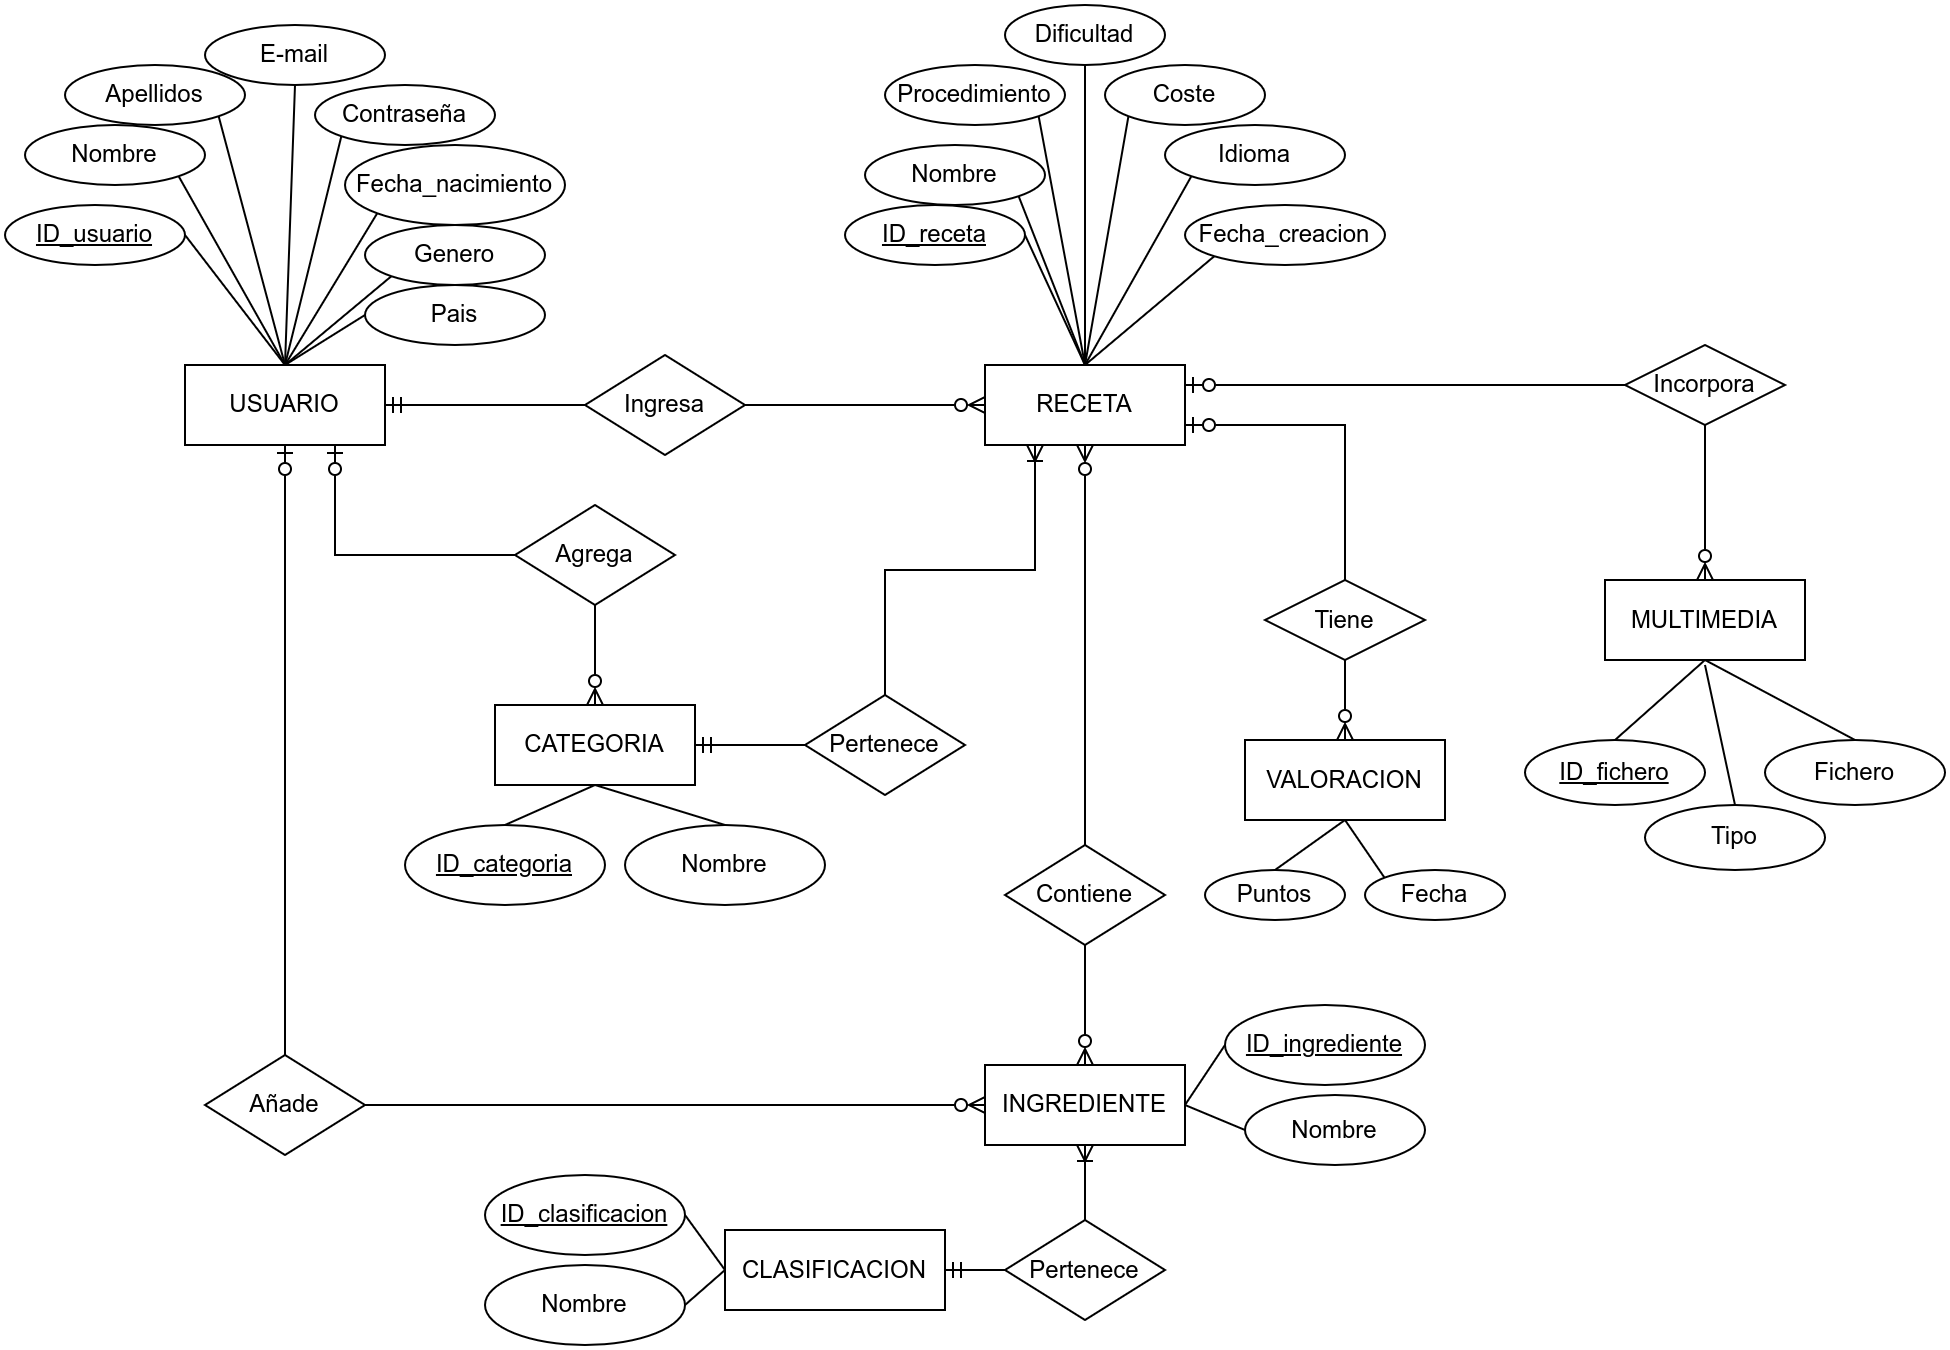
\includegraphics[width=\linewidth]{Actividad_2_entidad_relacion.png}

Este diseño se usará para realizar posteriormente la base de datos.


\section{Diagramas de caso de uso}
Teniendo en cuenta las funcionalidades exigidas que debe tener la aplicación de la \textbf{AIC}, junto con los requisitos que hemos visto previamente, es importante determinar los casos de uso que deben existir.

Para ellos, se han realizado distintos diagramas de uso que se expondrán a continuación junto con la funcionalidad exigida:

\vspace{-1em}
\begin{enumerate}[label=\alph*)]
    \item Registrar el usuario a la plataforma de la AIC.

    \begin{center}
        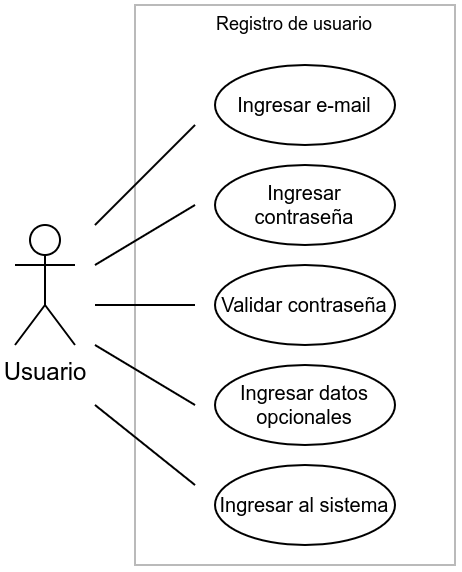
\includegraphics[width=0.3\linewidth]{casos/registro.png}
    \end{center}


    \item Autenticar usuario al ingresar a la aplicación de la AIC.

    \begin{center}
        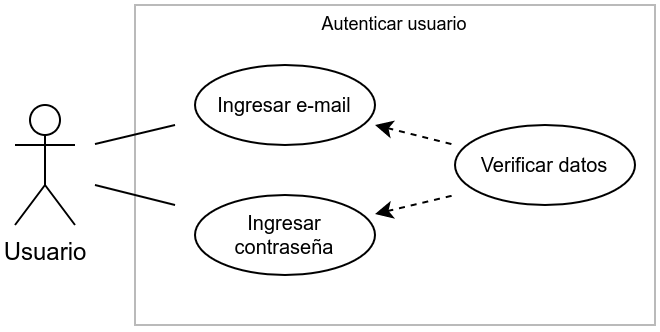
\includegraphics[width=0.5\linewidth]{casos/autenticar.png}
    \end{center}

    \item Cargar la receta, con todos sus aspectos asociados (categoría, lista de
    ingredientes, procedimiento, dificultad, costo, etc.)

    \begin{center}
        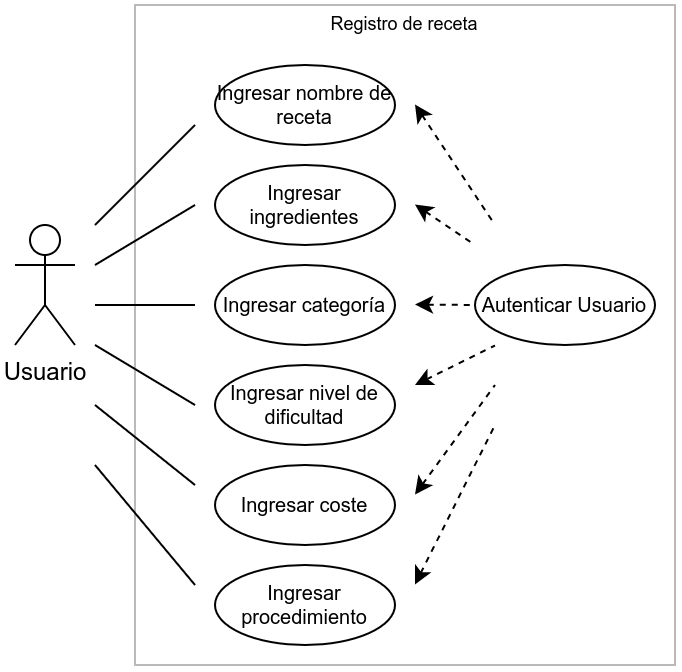
\includegraphics[width=0.5\linewidth]{casos/ingresar_receta.png}
    \end{center}


    \item Buscar recetas en base a distintos aspectos: clase de receta, tipo de ingrediente de base, nivel de dificultad, costo de la receta.

    \begin{center}
        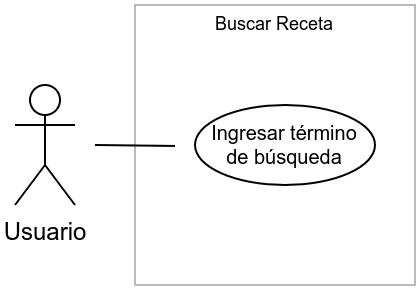
\includegraphics[width=0.4\linewidth]{casos/buscar_receta.png}
    \end{center}


    \item Visualizar resultados de búsqueda.

    \begin{center}
        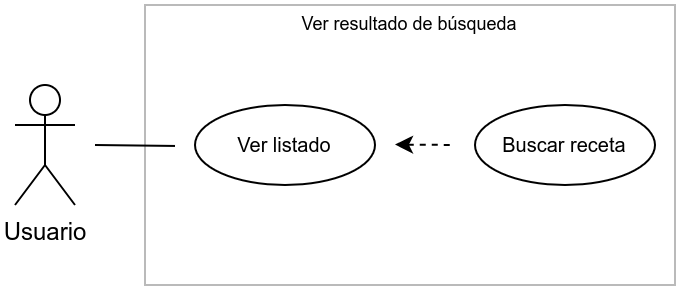
\includegraphics[width=0.5\linewidth]{casos/listado_receta.png}
    \end{center}

    \item Visualizar la información sobre cada receta.

    \begin{center}
        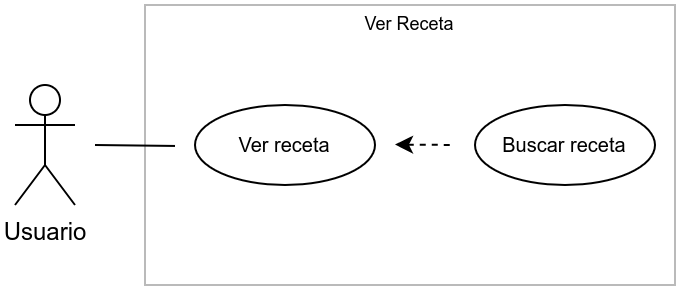
\includegraphics[width=0.5\linewidth]{casos/ver_receta.png}
    \end{center}

    \item Compartir receta en las redes.

    \begin{center}
        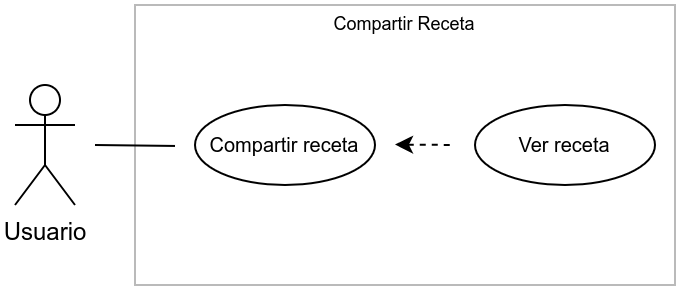
\includegraphics[width=0.5\linewidth]{casos/compartir_receta.png}
    \end{center}

    \item Valorar receta (de 1 a 5 estrellas).

    \begin{center}
        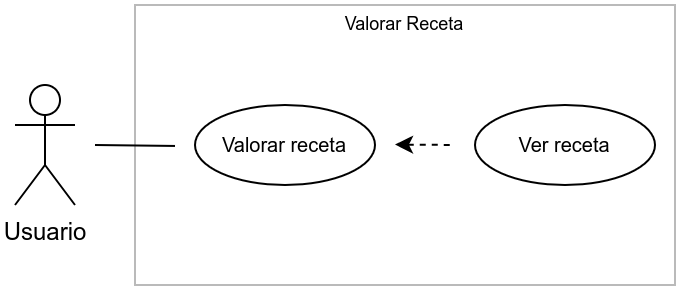
\includegraphics[width=0.5\linewidth]{casos/valorar_receta.png}
    \end{center}
\end{enumerate}

Tal como se puede ver, varios de los casos de uso dependen, a su vez, de otros casos de uso que pertenecen a otras funcionalidades.

Unificando estos casos de uso, junto con los requisitos explayados previamente, nos servirán para poder comenzar a detallar cómo queremos que sea el interfaz de la aplicación para la \textbf{AIC} en pasos sucesivos, y en última instancia comenzar con la programación de la aplicación.



\chapter{Conclusiones}
Tal como se ha podido ver a lo largo del documento, la obtención de los requisitos funcionales no es una tarea trivial y es por eso que es necesario entender las funcionalidades que \textbf{AIC} desea para su plataforma web.

Tras las reuniones realizadas con ellos, el posterior análisis de la información obtenida, la identificación y separación de los requisitos hará que las tareas posteriores, durante el desarrollo de la aplicación web, requieran de menos esfuerzo por parte de los desarrolladores.

Por último, destacar que con la realización de los diseños conceptuales de datos y de los casos de uso también se ha conseguido adelantar parte del esfuerzo que tendrá que ser realizado en procesos posteriores para la base de datos y el diseño de interfaces.


\printbibliography[title={Referencias bibliográficas},heading=bibintoc]

\end{document}
